\documentclass[letterpaper,11pt]{article}

\usepackage[margin=1.0in]{geometry}
\usepackage{amsmath}
\usepackage{amsthm}
\usepackage{amsfonts}
\usepackage{algorithm2e}
\usepackage{url}
\usepackage{fancyhdr}
\usepackage{blkarray}
\usepackage{graphicx}
\usepackage{csquotes}
\usepackage{cite}
\pagestyle{fancy}
\lhead{Algorithmic-Trading Summary --- Fall 2018}
\rhead{}


\begin{document}
\thispagestyle{plain}
\noindent{Algorithmic-Trading Summary --- Fall 2018}

\noindent{Alex Thomas}

\noindent{Colgate University} \\

\noindent\textbf{Algorithmic-Trading - Simple Moving Average - Application: Dual Moving Average}

\section*{Introduction }

Simple Moving Average (SMA) is an elementary AT strategy. Because of this, it is also the most commonly available tutorial online. The most common application of SMA is found in dual moving average \cite{AlmeidaTeixeira}, which utilizes two different averages that indicate momentum swings in the market.

\section*{Motivations and Measures}

Simple moving average looks at a rolling average of a specified window. Mathematically this can be defined as: SMA($t$)$ = 1/n \sum_{i=t-n}^{t}x(i)$ \cite{AlmeidaTeixeira} In words, this gets the average price over a specified window of time for a specified function. In context to the stock market, SMA can be applied for both short term and long term averages, with the former under an hour while the latter can be over hundreds of days. In application to the stock market and closing prices, this creates an average closing price for a specified amount of time, which gives an indicator of price swings in that period of time.

\section*{Key Techniques}

The dual moving average technique is one of the most widely used techniques. It works by taking two different SMA's - a short window and a long window. In our implementation, a 40 day window and 200 day window were chosen, giving insight into a strategy that uses longer averages. The short window crossing below the long window gives a buy signal reinforced by high trading volumes while the opposite is considered bearish and gives a sell signal. Figure 1 demonstrates this strategy graphically. The purple triangles represent a buy signal, while the black triangles represent sell signals. 

\begin{figure}[ht!]
\centering
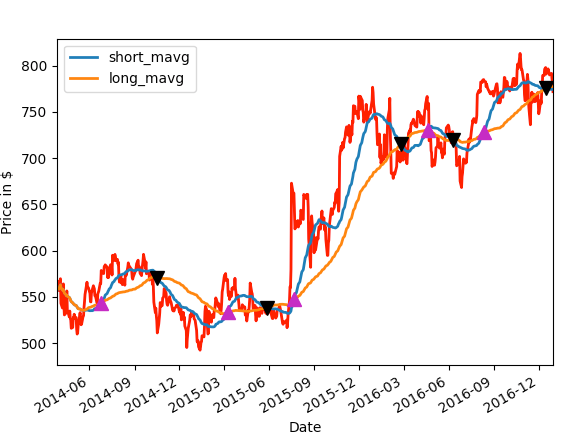
\includegraphics[width=90mm]{SMA_Google.png}
\caption{Dual Moving Average Strategy applied to GOOG \label{overflow}}
\end{figure}

\section*{Analysis}

\subsection*{Effectiveness}
Due to the nature of SMA, which generally looks at long periods of time to highlight trends, this can induce a lagged effect to the buy and sell orders. This lagged effect can be fixed by looking at an Exponential Moving Average analysis \cite{Ehlers}. In our implementation, the short window looks over a period of 40 days while the long window is 200 days. For a meaningful change to register it requires multiple days of continued poor or good performance for a sizable change to register. For example, given a recent downtrend in a particular stock over the last 7 days, the shorter window wouldn't feel that effect yet Therefore, this can cause a lagged effect, making this algorithm not very effective. Figure 1's sell signal in 2016-03 demonstrates this effect.

\subsection*{Runtime}
The components to consider for this strategy include pulling stock data into a Pandas data frame and calculating rolling means from the data-frame and marking their differences. Pandas is a python data analysis package and is perhaps the most powerful open source data analysis or manipulation tool available. For each calculation, it has to scrape through the entire data-frame at a rolling window, giving a linear runtime.

\subsection*{Quality Metric}
The strategy is tested against a baseline long position of a given stock. For our implementation stocks AAPL, GOOG, DIS, FB, INTC were chosen. None of the chosen stocks outperformed the baseline performance. Facebook had by far and away the closest performance with only a -0.64\% performance against the baseline. Google had the worst performance and ended up with a -30.25\% performance with the strategy actually going negative profit.

\subsection*{Space / Memory implications}
The only space for SMA required is the data-frame, which is very reasonable.

\section*{Conclusion}

SMA is a simple AT strategy that looks at rolling window averages of closing prices for a particular stock. SMA is often applied in this dual moving average implementation where both short and long windows crossing generates buy and sell orders. However, it's performance against a baseline long position is not good, as the baseline long position for the stocks chosen always outperforms the strategy. 

\section*{Implementation}
\begin{verbatim}
def execute(stock, start_date, end_date):
    stock = stockDataRetriever(stock, start_date, end_date).getStock()

    # Initialize the short and long windows and buy sell in df
    short_window = 40
    long_window = 100
    
    # set Pandas df with stock data
    df = pd.DataFrame(index=stock.index)

    # Create short and long simple moving average 
    df['short_movin_average'] = df.movingWindow(short_window)
    df['long_moving_average'] = df.movingWindow(long_window)
    
    # mark signal based on comparison of the two averages
    df['signal'] = df.compare(short_moving_average, long_moving_average,1,0)
    
    # when signal changes from 1 to 0 or 0 to 1 - is a buy or sell
    df['positions'] = df['signal'].diff()

\end{verbatim}

\bibliographystyle{plain}
\bibliography{References}

\end{document}